\newpage
\chapter{DISEÑO DEL SISTEMA DE INFORMACIÓN}
	\vspace{2cm}	
	\begin{center}
	{\Large \textbf{FASE DE DESARROLLO} \par}
	\end{center}
	\vspace{5cm}
	
	\begin{center}
	\Huge \textbf{DSI}\par
	\end{center}


%\newpage
%
%\section{DSI 3: DISEÑO DE CASOS DE USO REALES}
%
%\subsection{Caso de Uso 1.1} 
%
%\subsubsection{Diagramas de Interacción (Comunicación y Secuencia)} 
%
%\subsubsection{Diagramas de Estados de las Clases} 
% 
%\subsubsection{Diagramas de Actividades} 
%
%
%\subsection{Caso de Uso 1.2}


\newpage
\section{DSI 4: DISEÑO DE CLASES}
\subsection{Diagrama de Clases}
\subsubsection{Museo}
\begin{figure}[H]
\centering
\centerline{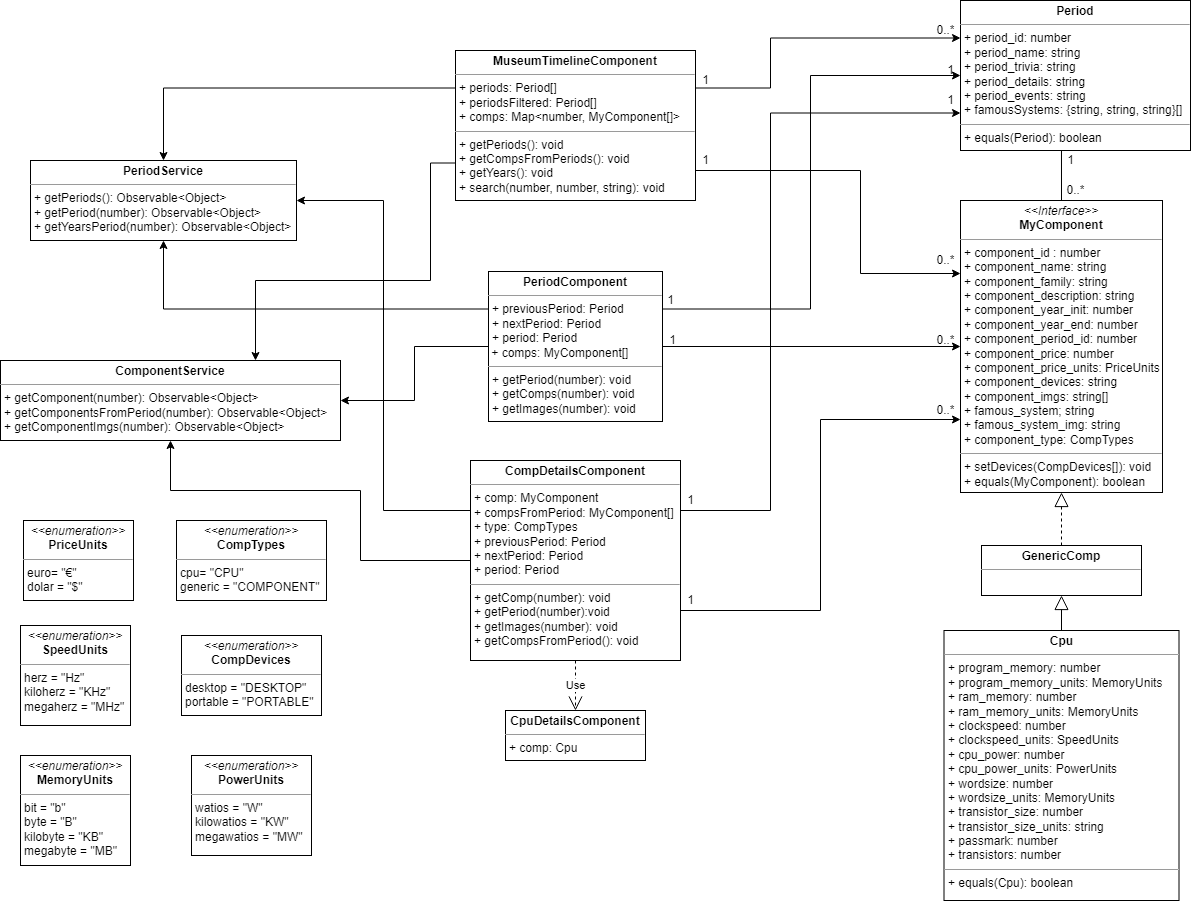
\includegraphics[scale=0.4]{dis-clases-museo}}
\caption{Diseño de clases: diagrama de clases del museo}
\end{figure}
\subsubsection{Administración del museo}
\begin{figure}[H]
\centering
\centerline{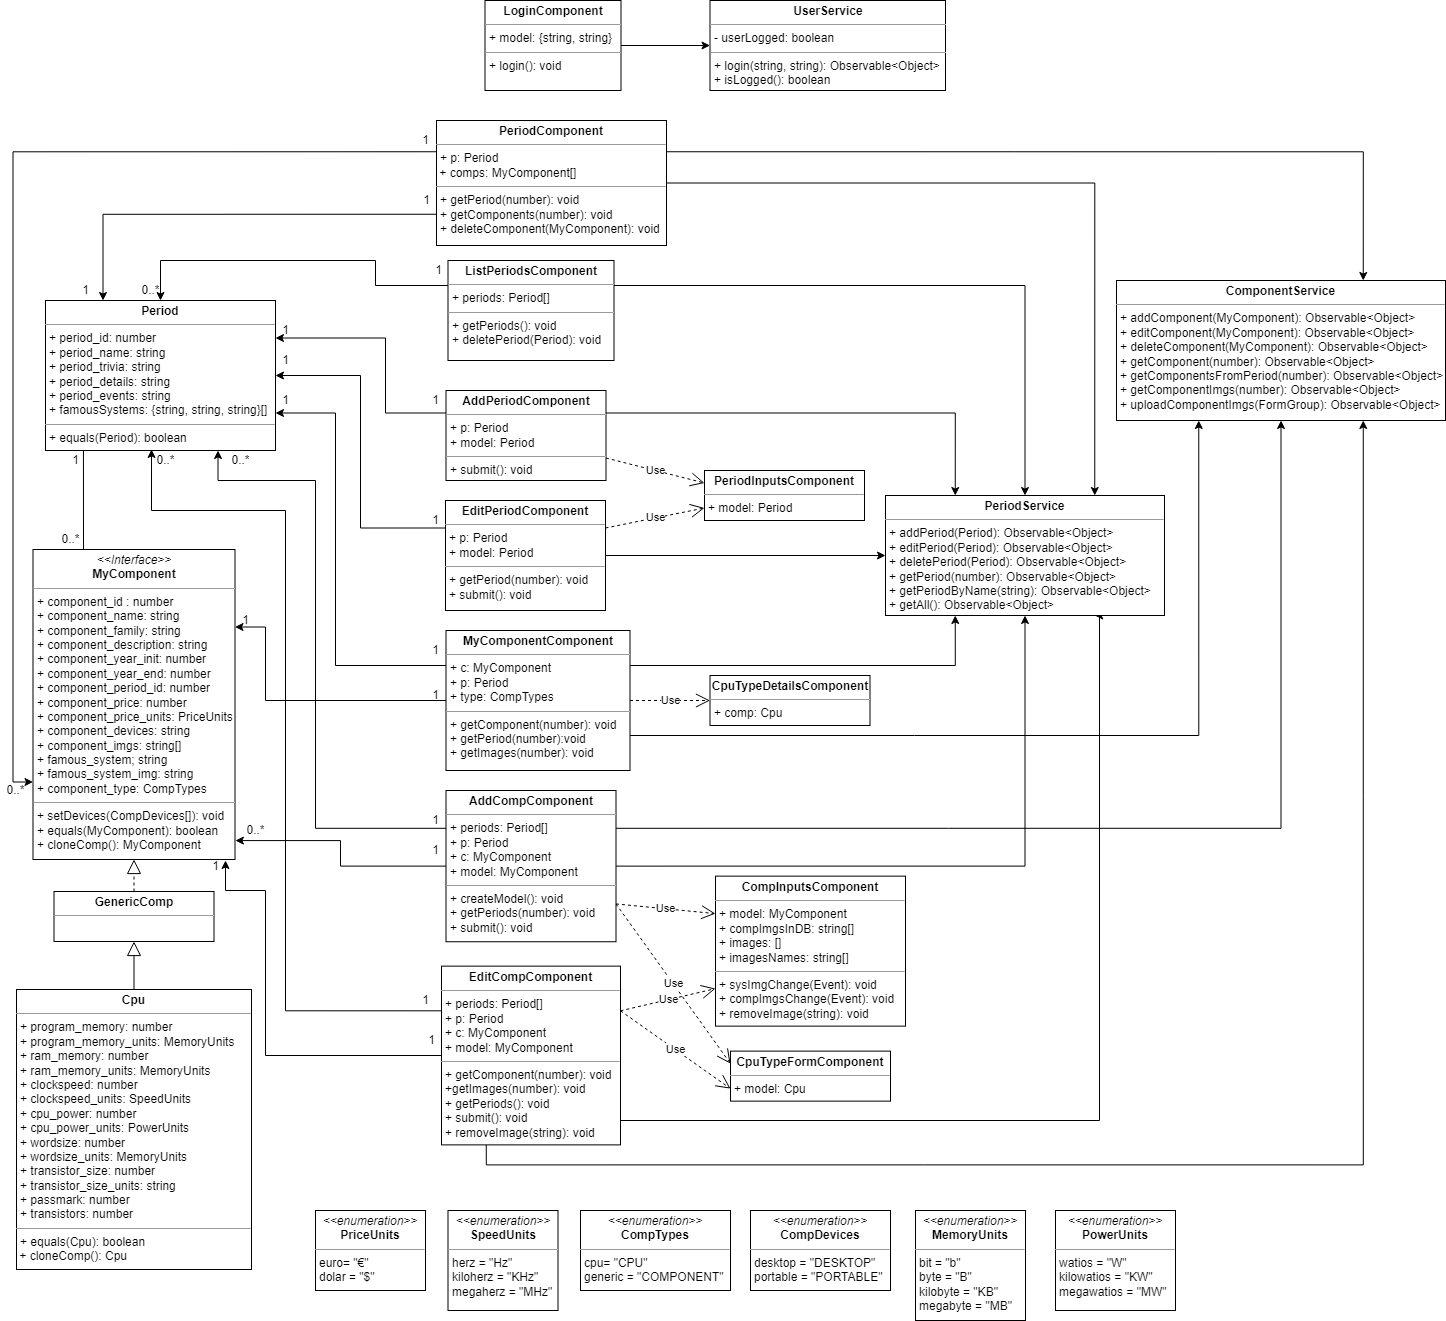
\includegraphics[scale=0.4]{dis-clases-admin}}
\caption{Diseño de clases: diagrama de clases de la administración del museo}
\end{figure}

\newpage
\section{DSI 5: DISEÑO DE LA ARQUITECTURA DE MÓDULOS DEL SISTEMA}

\subsection{DSI 5.1 Diseño de Módulos del Sistema}

\subsection{DSI 5.2 Diseño de Comunicaciones entre Módulos}

\subsection{DSI 5.3 Revisión de la Interfaz de Usuario}
A continuación, se muestran las interfaces definitivas de la aplicación web.
\subsubsection{Museo}
\begin{figure}[H]
\centering
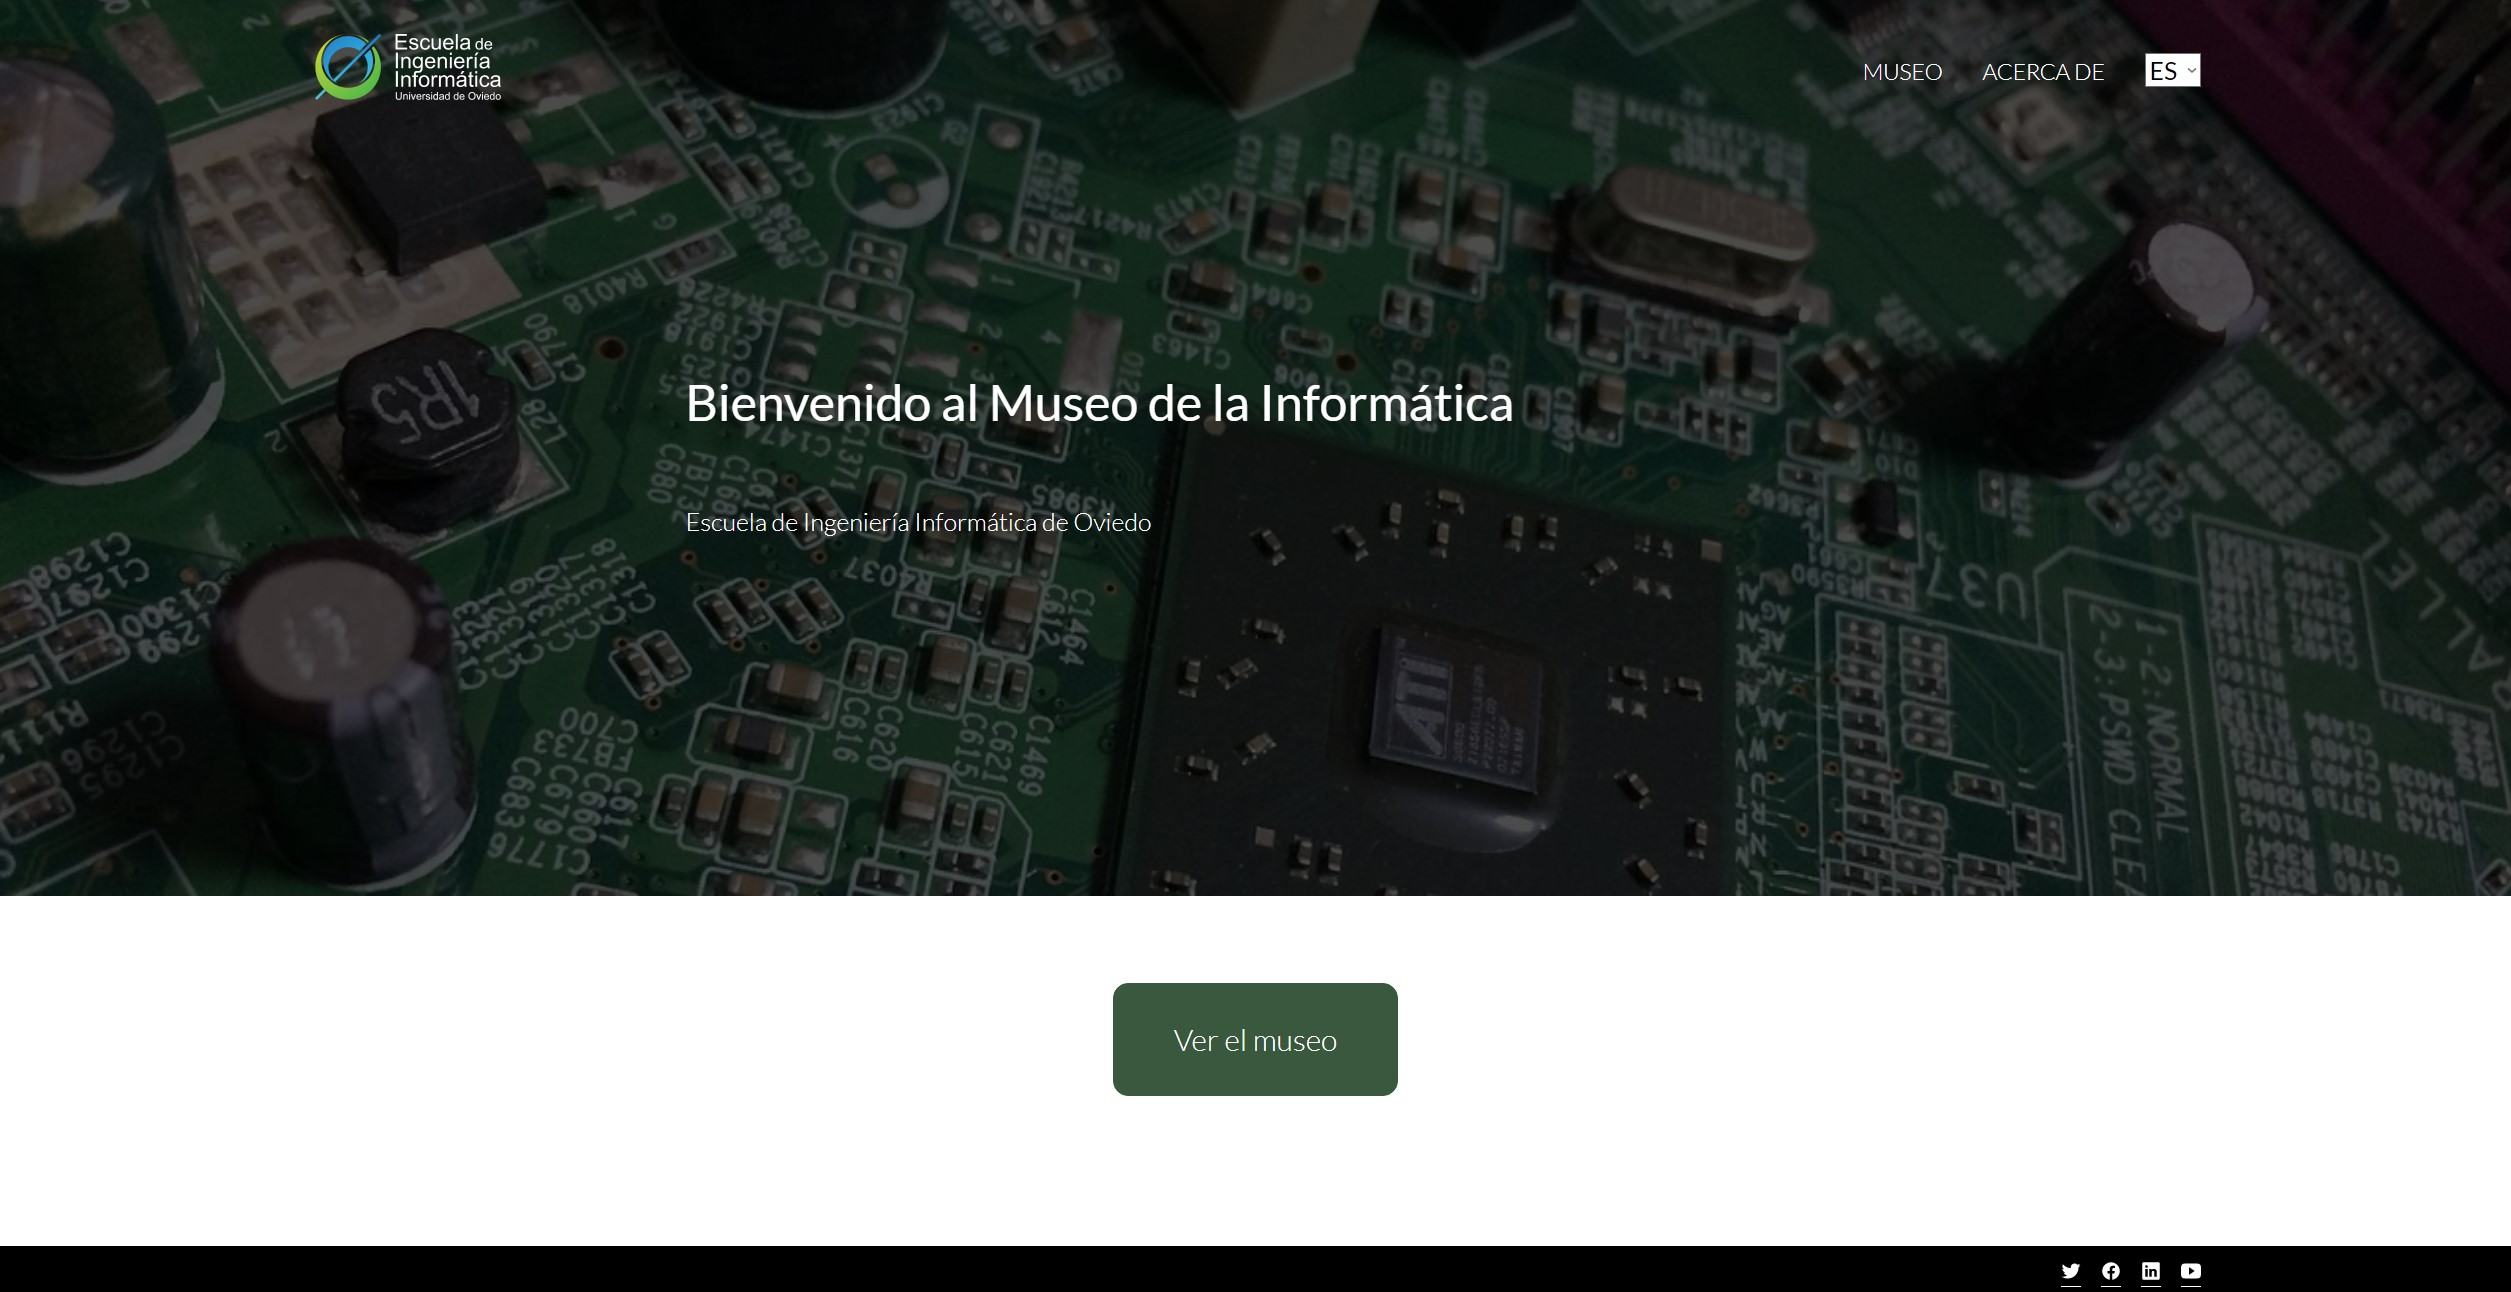
\includegraphics[scale=0.25]{homeIUDef}
\caption{Página de inicio}
\end{figure}
\begin{figure}[H]
\centering
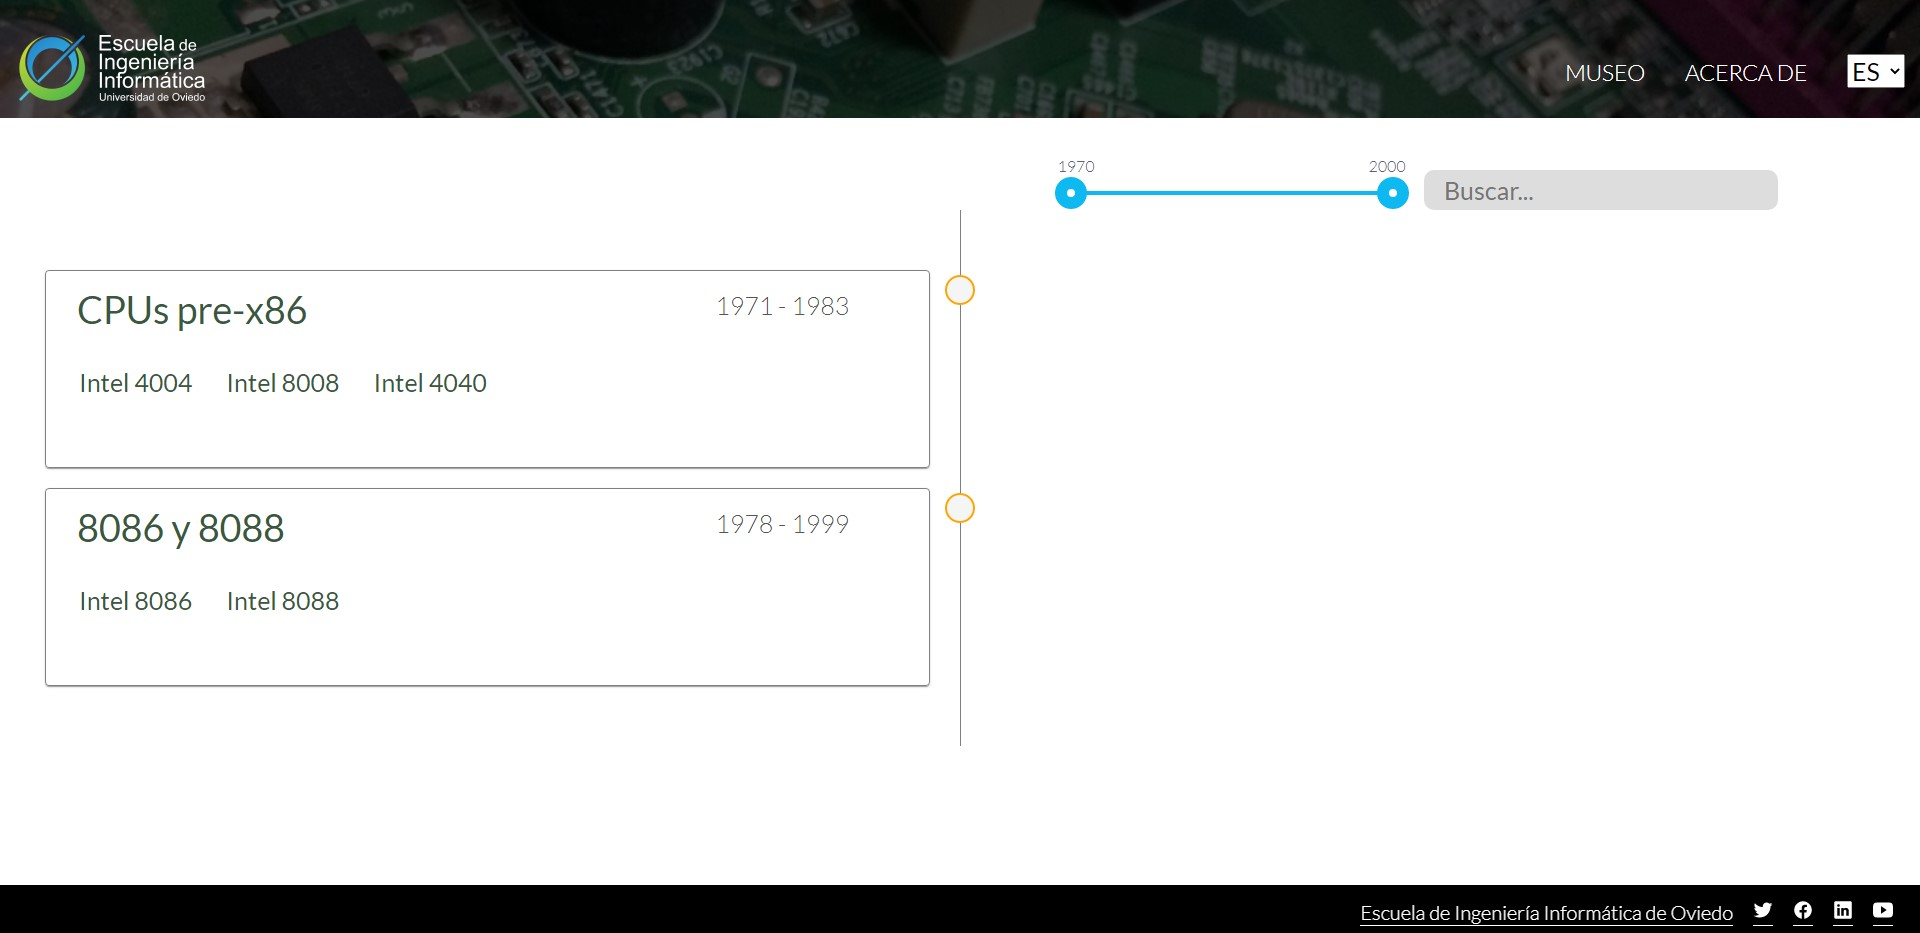
\includegraphics[scale=0.25]{museoIUDef}
\caption{Página de la vista general del museo}
\end{figure}
\begin{figure}[H]
\centering
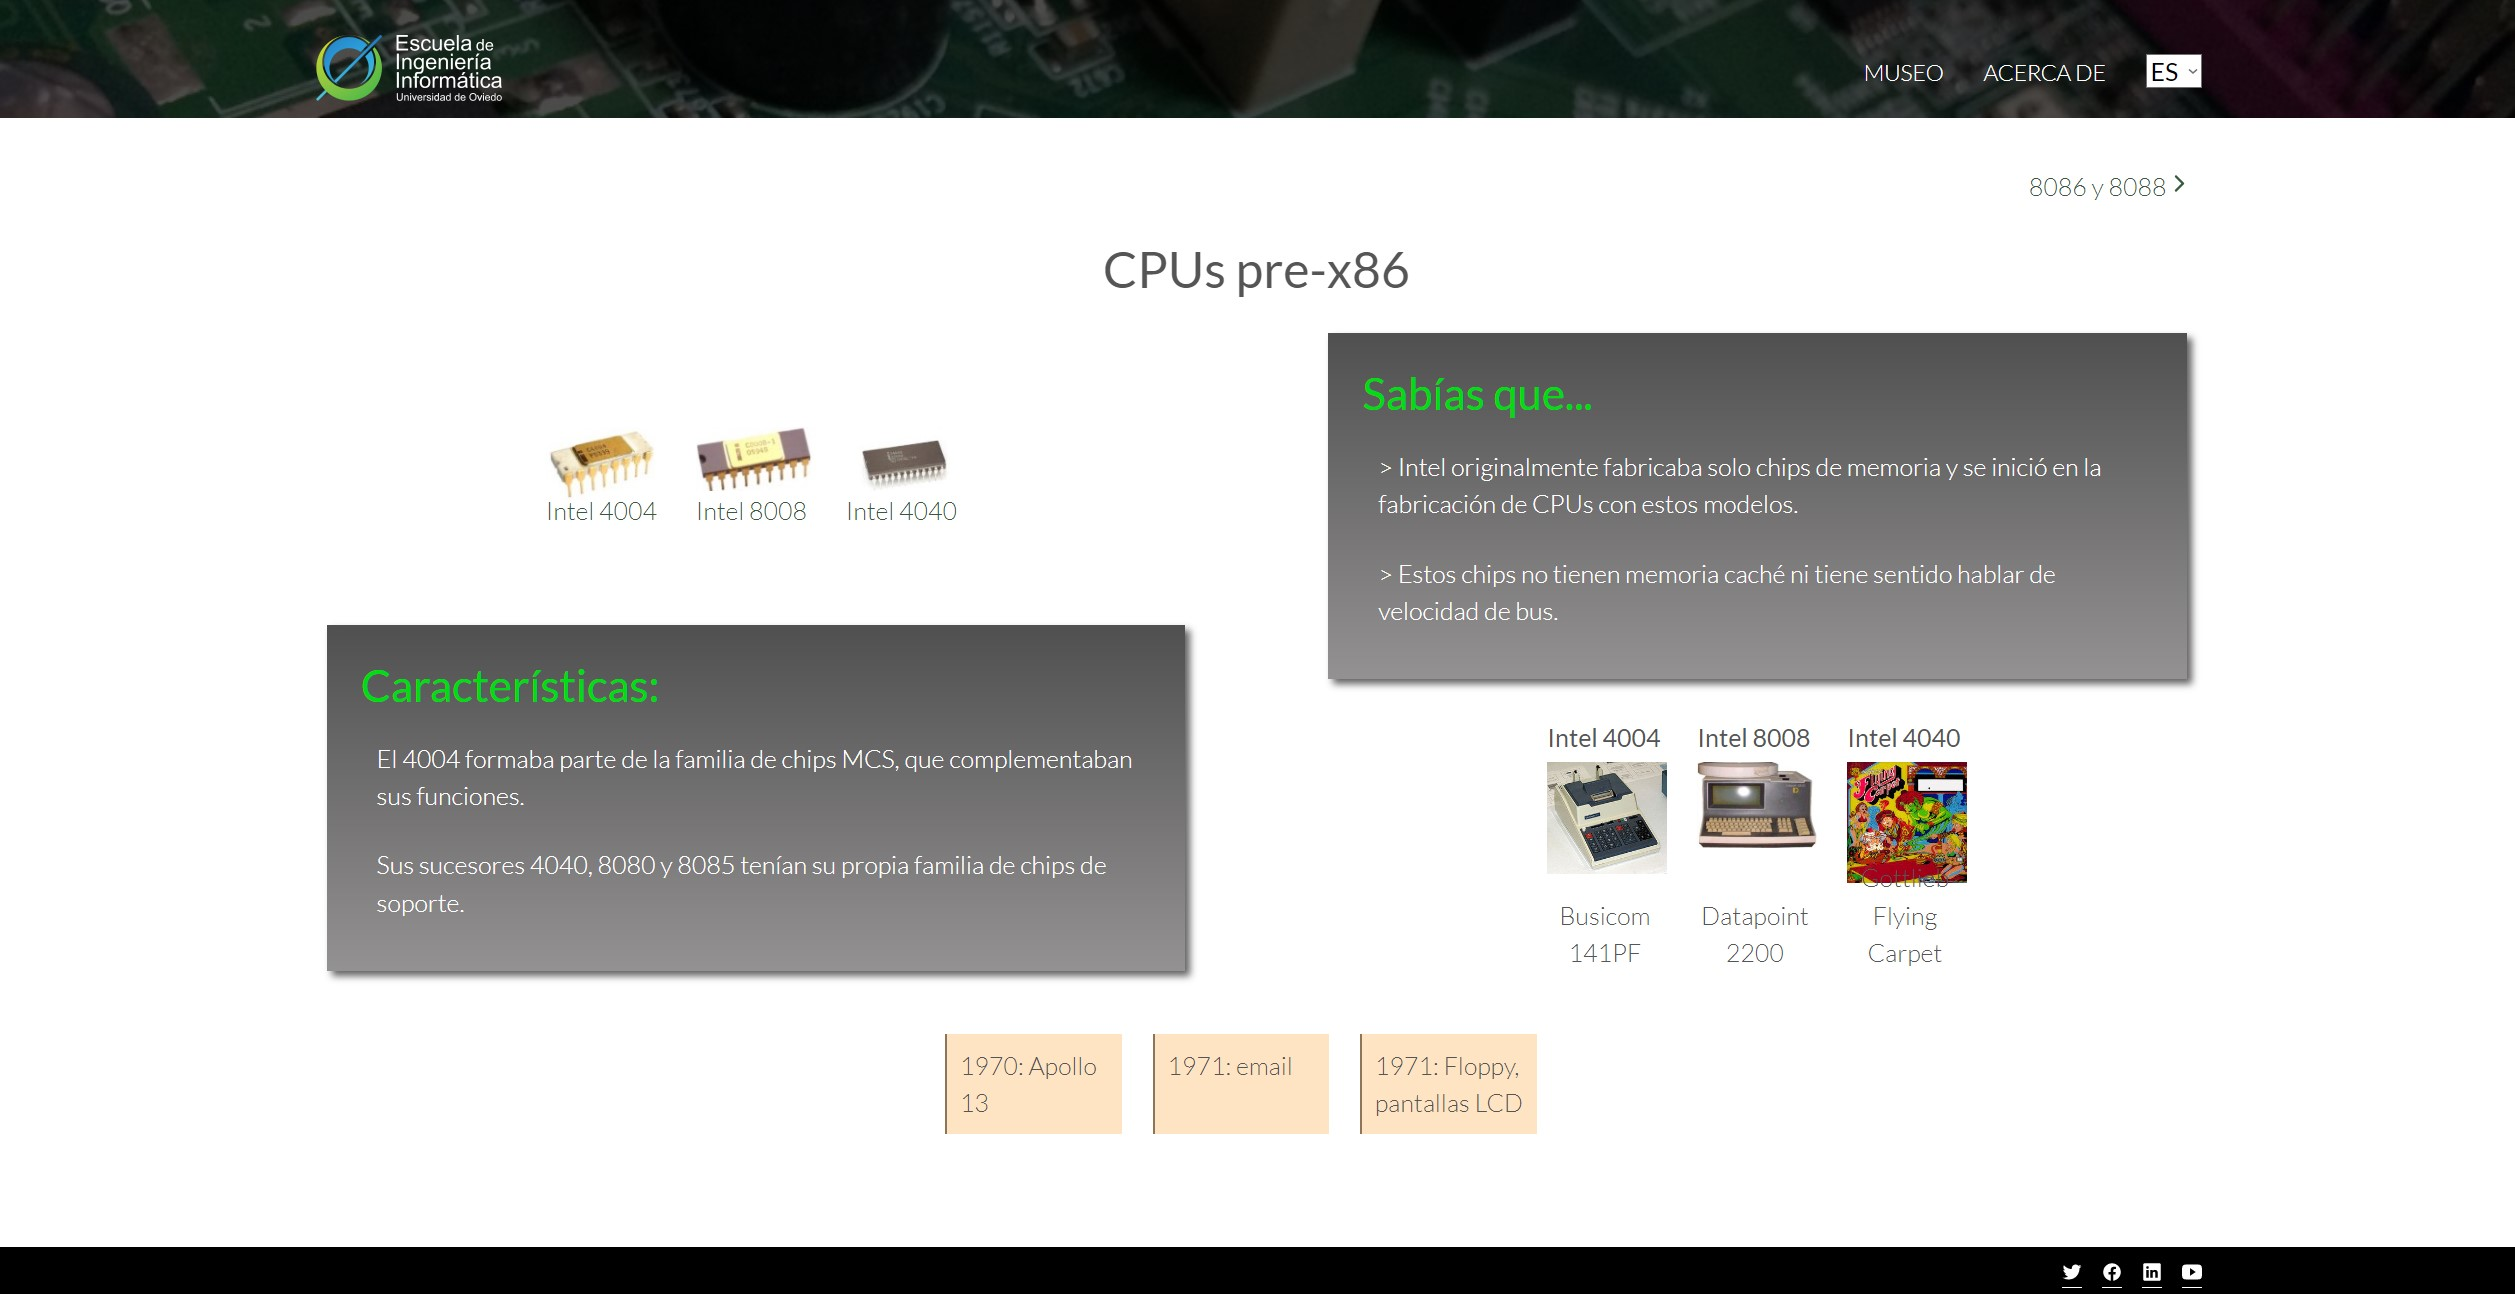
\includegraphics[scale=0.25]{periodoIUDef}
\caption{Página de detalles del periodo (museo)}
\end{figure}
\begin{figure}[H]
\centering
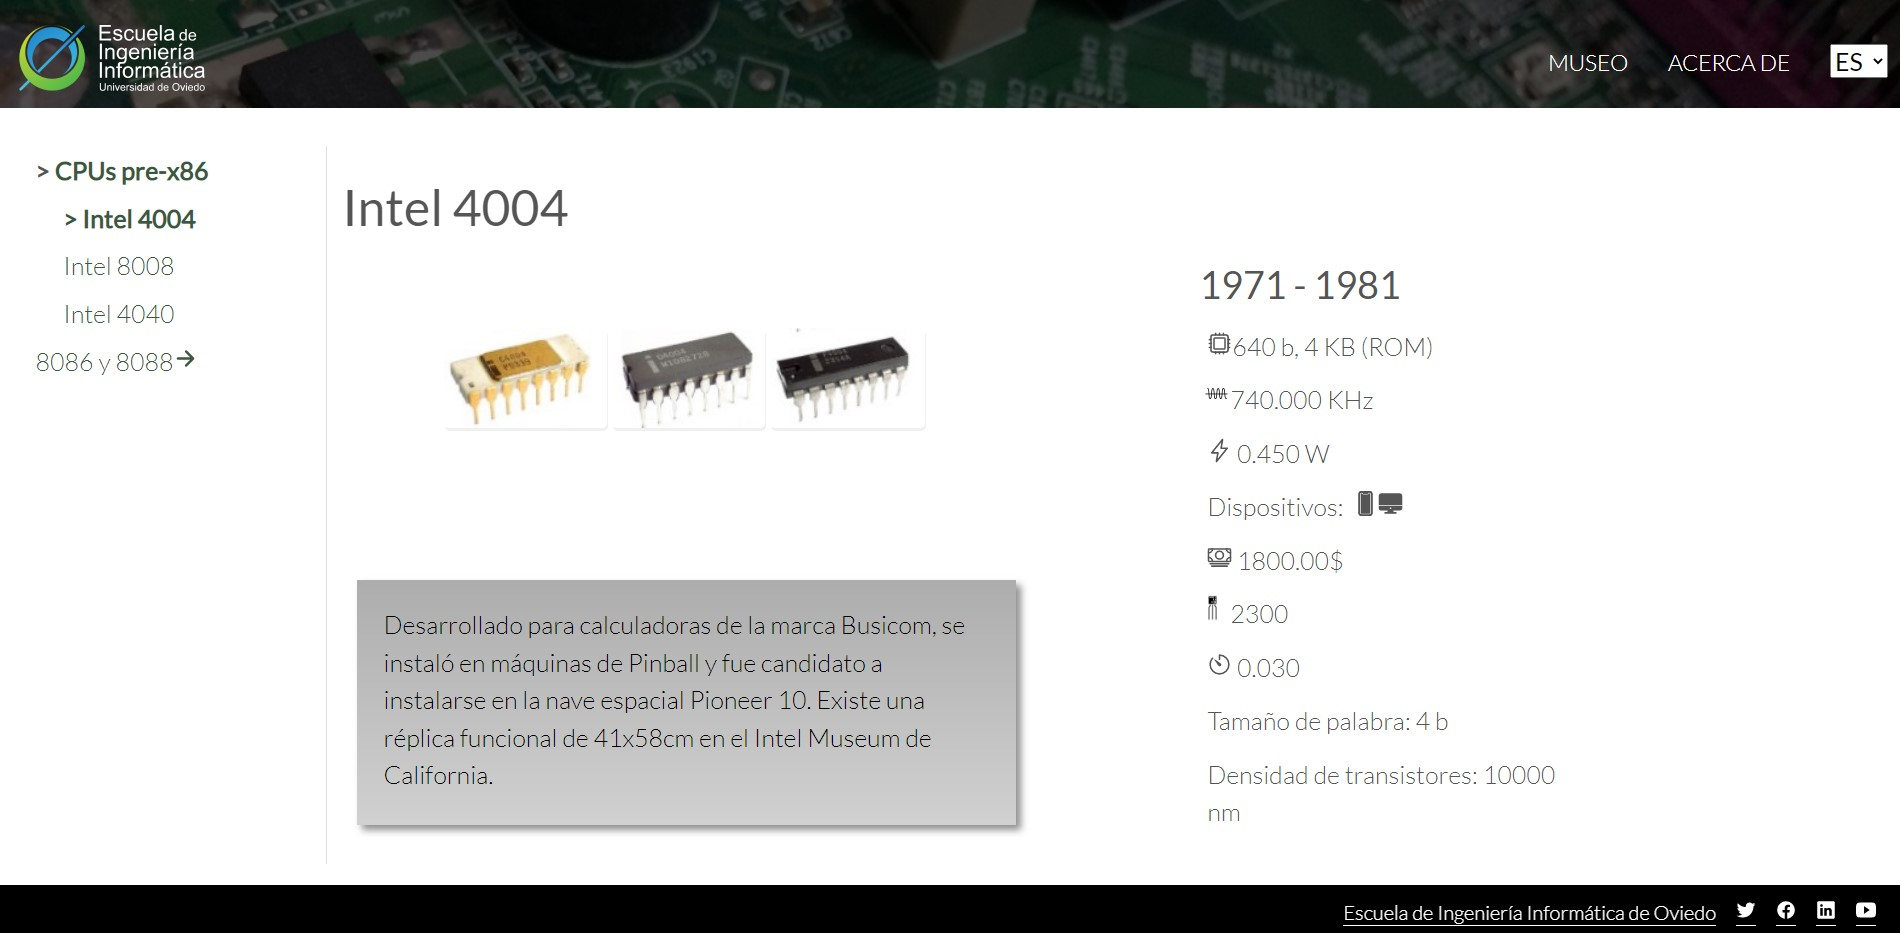
\includegraphics[scale=0.25]{piezaIUDef}
\caption{Página de detalles del componente (museo)}
\end{figure}

\subsubsection{Administración del museo}
\begin{figure}[H]
\centering
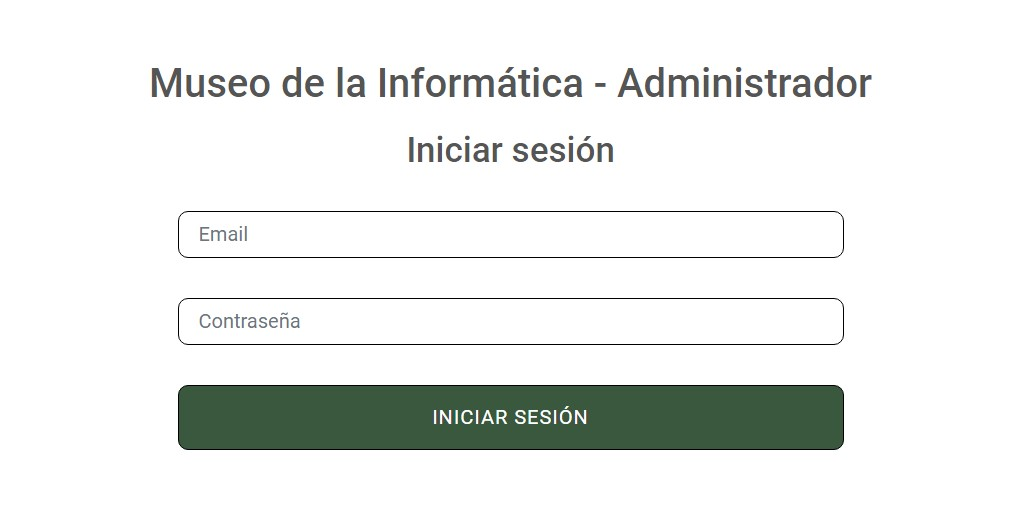
\includegraphics[scale=0.55]{loginIUDef}
\caption{Página de inicio de sesión}
\end{figure}
\begin{figure}[H]
\centering
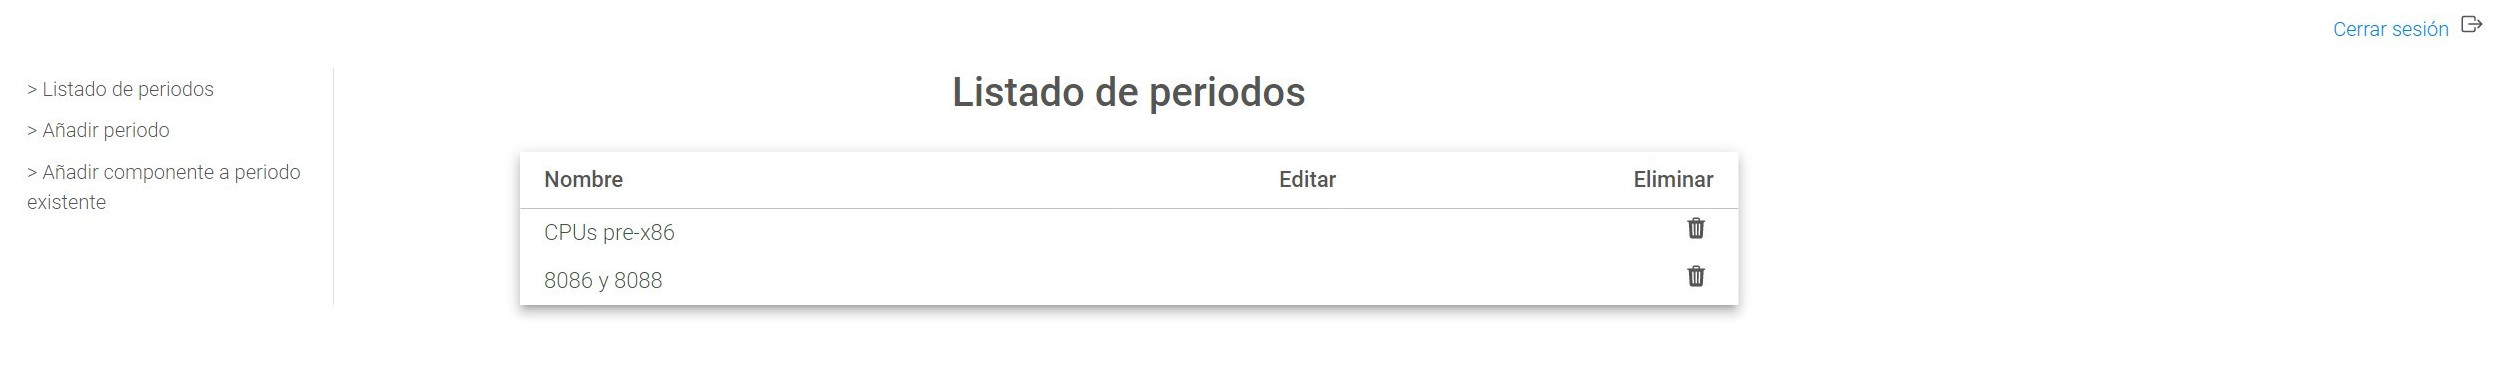
\includegraphics[scale=0.35]{listadoPeriodosIUDef}
\caption{Página de listado de periodos}
\end{figure}
\begin{figure}[H]
\centering
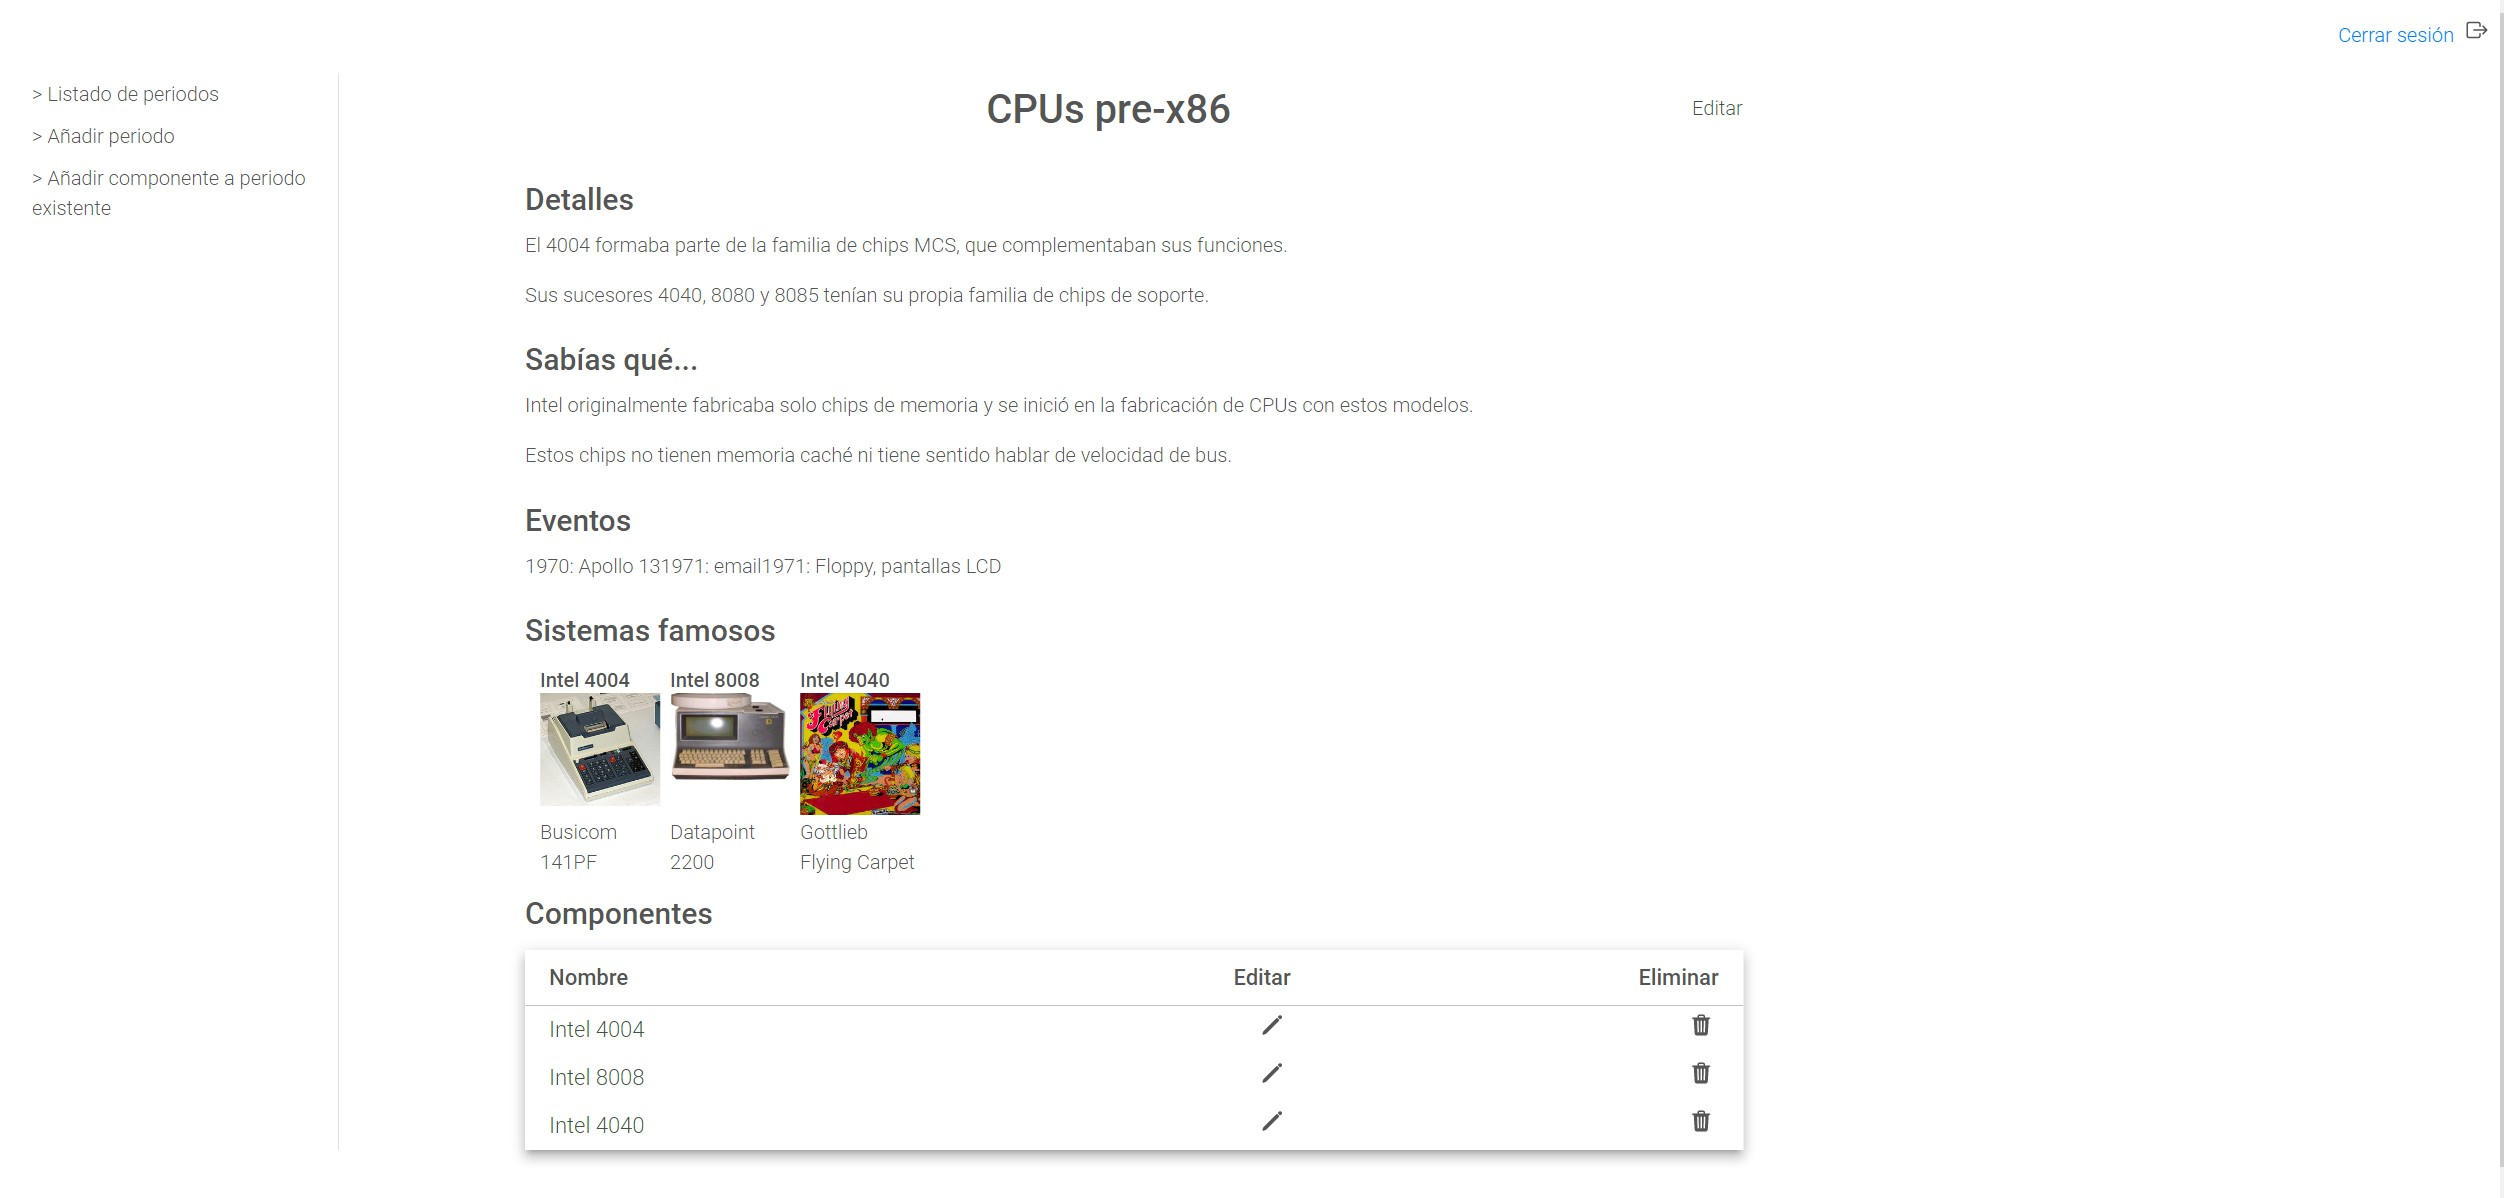
\includegraphics[scale=0.35]{periodoIU2Def}
\caption{Página de detalles de un periodo (administración)}
\end{figure}
\begin{figure}[H]
\centering
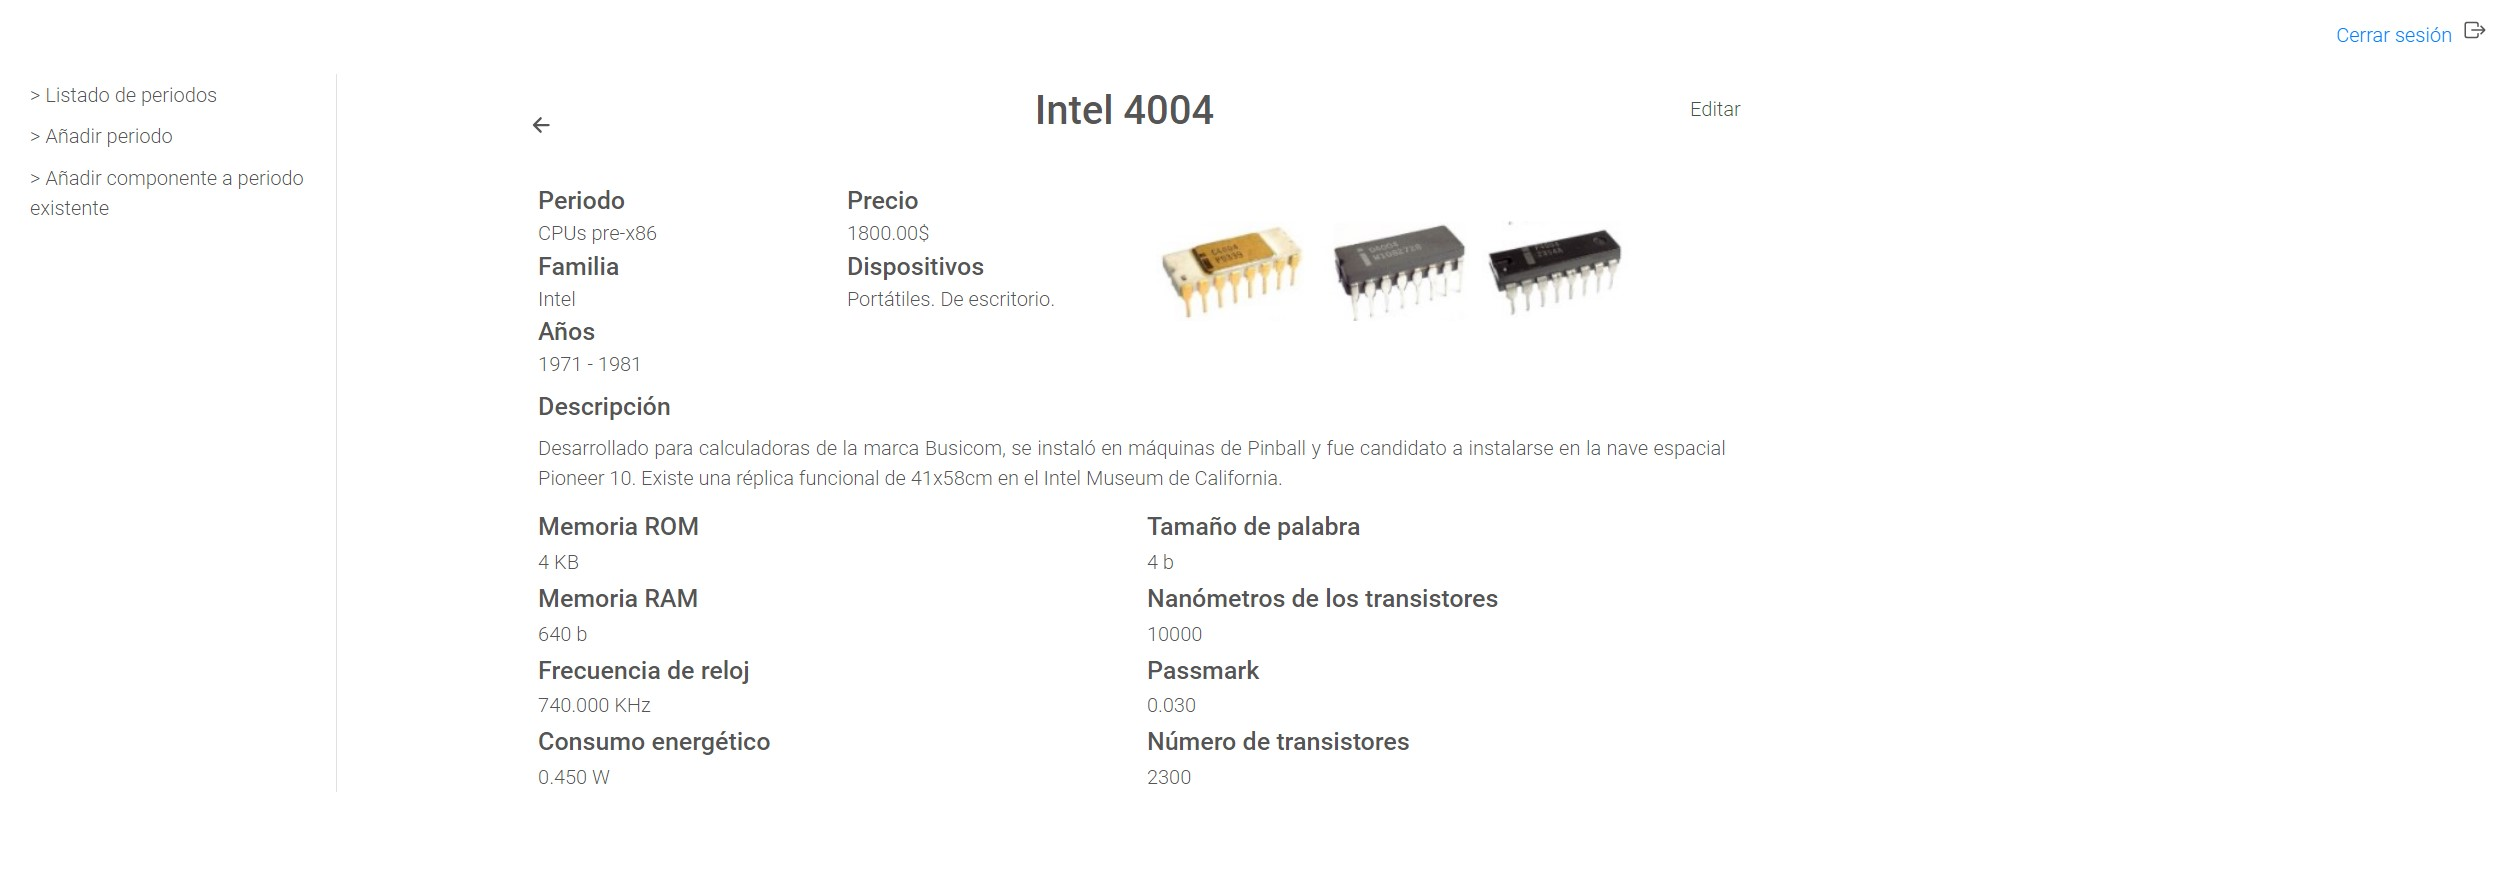
\includegraphics[scale=0.35]{compIUDef}
\caption{Página de detalles de un componente (administración)}
\end{figure}
\begin{figure}[H]
\centering
\includegraphics[scale=0.35]{añadirPeriodoIUDef}
\caption{Formulario para añadir un periodo}
\end{figure}
\begin{figure}[H]
\centering
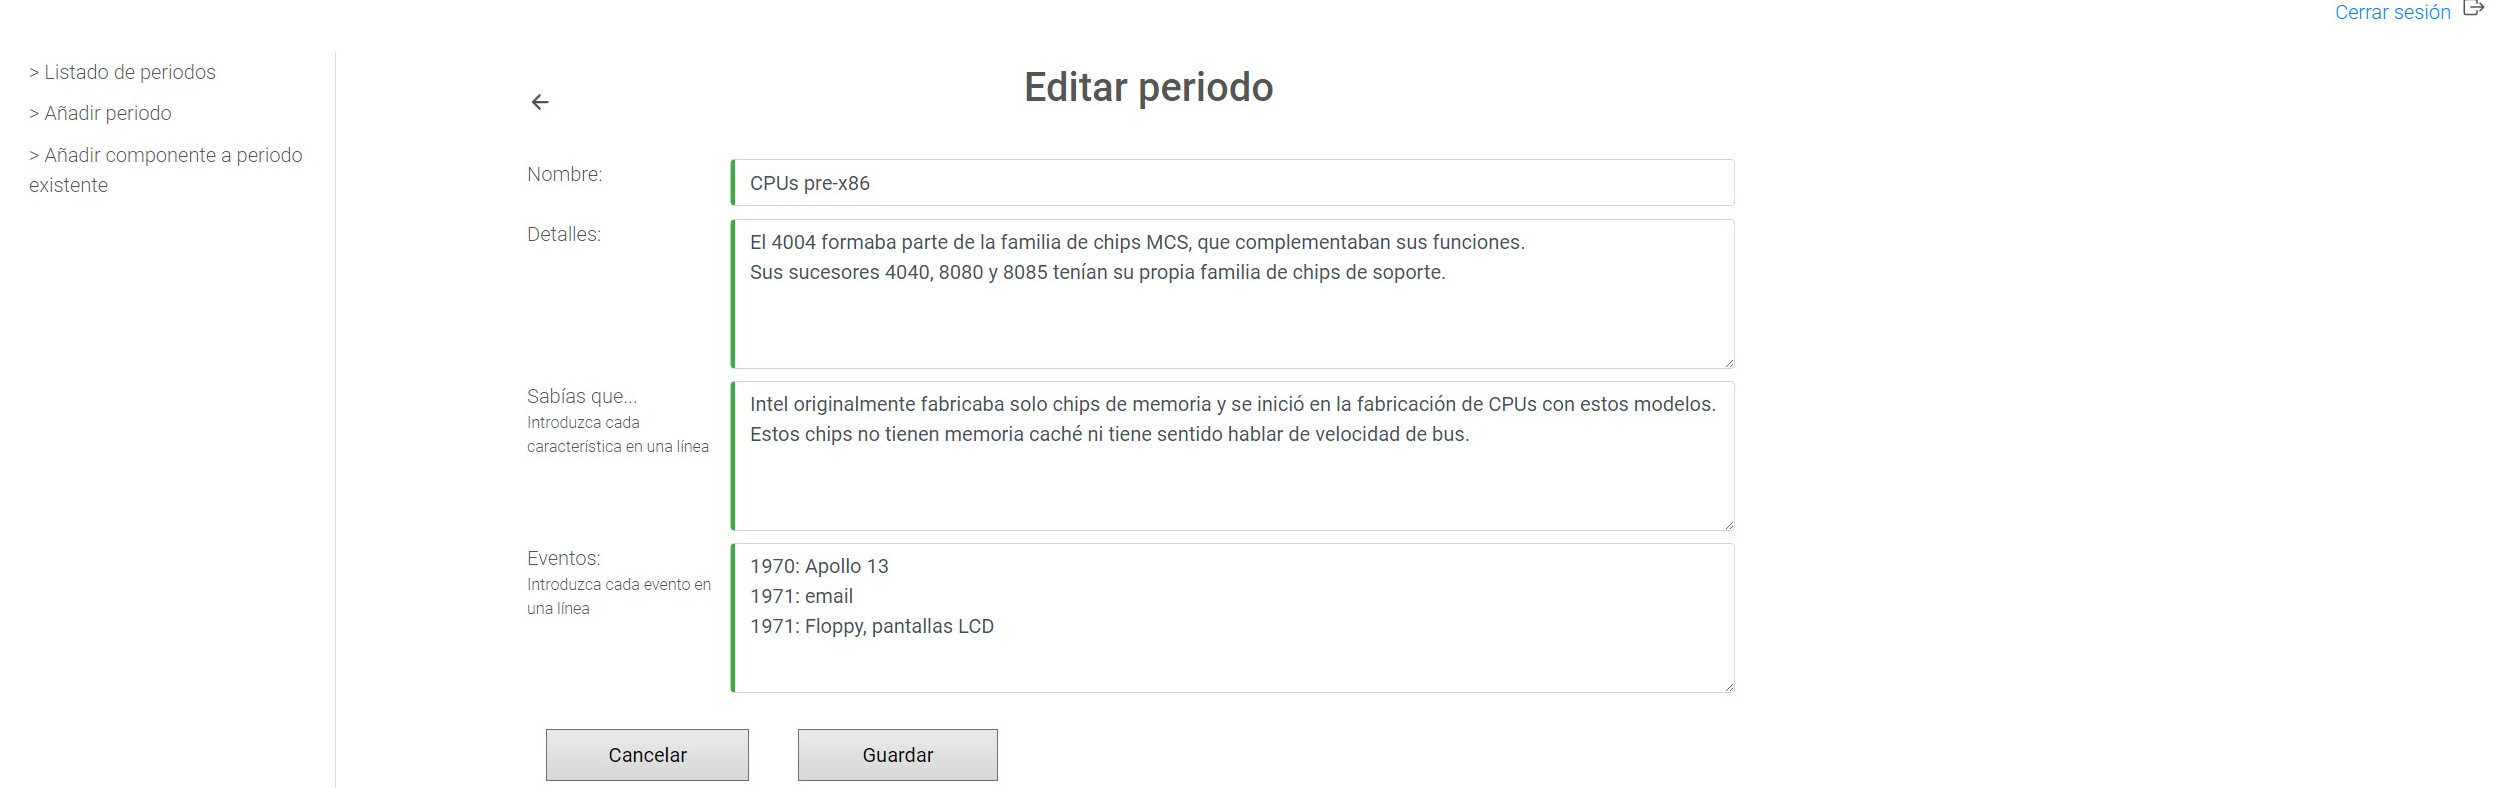
\includegraphics[scale=0.35]{editarPeriodoIUDef}
\caption{Formulario para editar un periodo}
\end{figure}
\begin{figure}[H]
\centering
\includegraphics[scale=0.35]{añadirCompIUDef}
\caption{Formulario para añadir un componente}
\end{figure}
\begin{figure}[H]
\centering
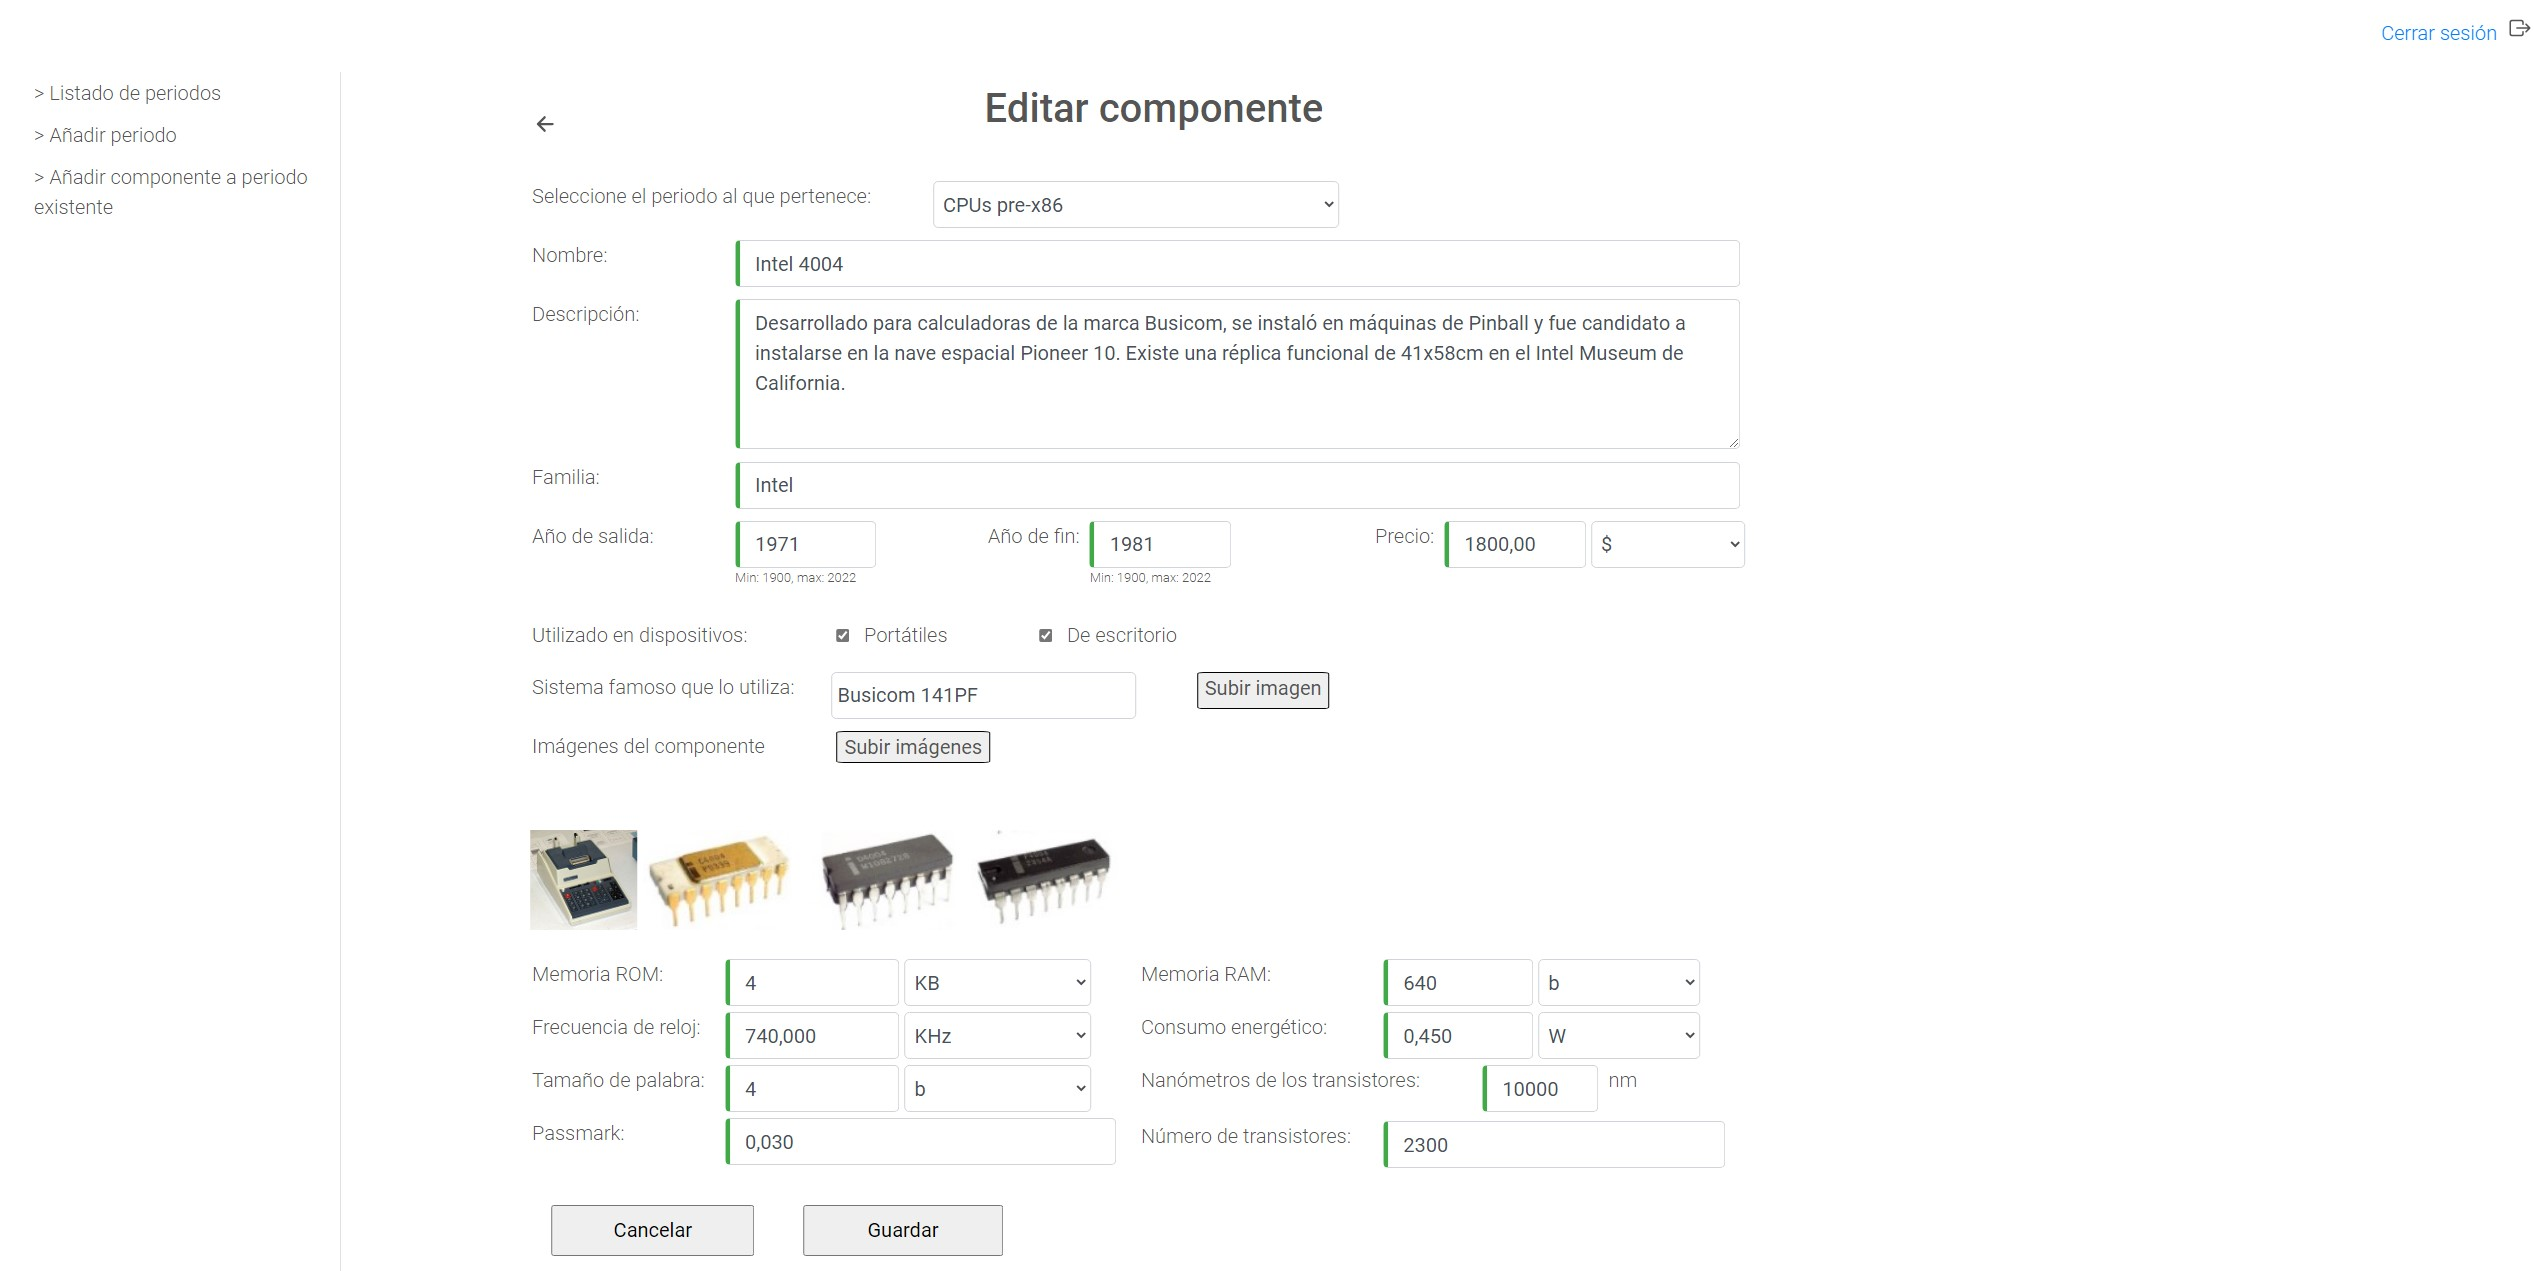
\includegraphics[scale=0.35]{editarCompIUDef}
\caption{Formulario para editar un componente}
\end{figure}



\newpage
\section{DSI 6: DISEÑO FÍSICO DE DATOS}

\subsection{Descripción del SGBD Usado} 
Se ha creado una base de datos relacional, utilizando MySQL 8 como sistema gestor de bases de datos, debido a su gran popularidad en todo el mundo y en el desarrollo de aplicaciones con Angular y PHP.
\par La base de datos creada es museo-eii, y se compone de cinco tablas: 
\begin{itemize}
	\item periods: alamcena toda la información relativa a un periodo.
	\item components: contiene los datos que serían comunes a cualquier tipo de componente idependientemente de su tipo, como nombre, año de salida, precio, ect.
	\item components\_images: asigna el conjunto de imágenes de cada componente.
	\item cpus: almacena los datos específicos de una CPU, como la memoria RAM, la velocidad de reloj o el tamaño de palabra. El identificador de esta tabla referencia al elemento correspondiente de la tabla components, simulando así una herencia en la base de datos. Esta herencia simulada hace que la base de datos sea fácilmente ampliable si se añade un tipo de componente que no sea una CPU, ya que bastaría con añadir una nueva tabla con los campos necesarios que también referencie a components.
	\item administrator: almacena los datos de inicio de sesión del administrador (email y contraseña cifrada). En caso de que hubiera más usuarios que tuviesen que iniciar sesión se habría creado una base de datos exclusiva para almacenarlos, pero como en este caso solo existe un administrador, he decidido incluir esta tabla en la base de datos existente para este proyecto.
\end{itemize}
\subsection{Integración del SGBD en Nuestro Sistema} 
Para integrar el sistema con la base de datos se han creado tres servicios en angular: uno para periodos, otro para componentes y el último para el usuario. Estos tres servicios utilizan la librería HttpClient de Angular, que permite realizar peticiones HTTP para obtener o enviar datos al lado del servidor, donde se encuentran los archivos PHP que contienen las consultas que han de realizarse sobre la base de datos.
\subsection{Diagrama E--R} 
A continuación se muestra el diagrama entidad-relación de la base de datos del sistema, museo-eii:
\begin{figure}[H]
\centering
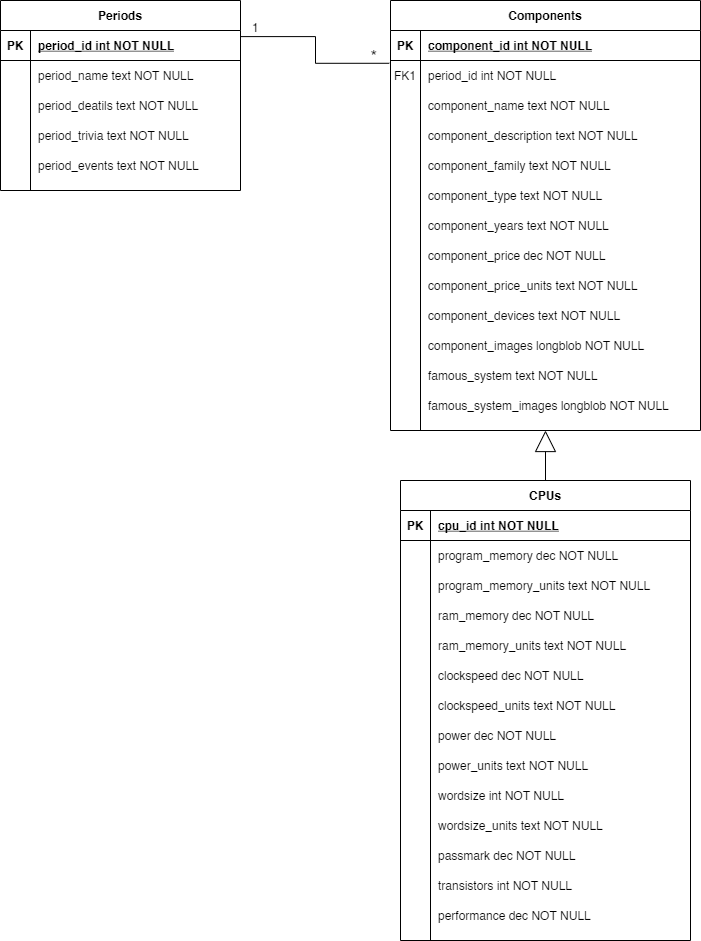
\includegraphics[scale=0.6]{diagrama_e-r}
\caption{Diagrama Entidad-Relación de la base de datos creada}
\end{figure}

\newpage
\section{DSI 9: DISEÑO DE LA MIGRACIÓN Y CARGA INICIAL DE DATOS}


\newpage
\section{DSI 10: ESPECIFICACIÓN TÉCNICA DEL PLAN DE PRUEBAS}

\subsection{Pruebas Unitarias} 

\subsection{Pruebas de Integración y del Sistema} 

\subsection{Pruebas de Usabilidad y Accesibilidad} 

\subsubsection{Diseño de Cuestionarios} 

\subsubsection{Actividades de las Pruebas de Usabilidad} 


\subsection{Pruebas de Accesibilidad} 

%\subsection{Pruebas de Rendimiento} 
